\documentclass[a4paper, 12pt]{article}

\usepackage{url}
\usepackage{graphicx}
\usepackage{caption}
\usepackage[section]{placeins}
\usepackage{fixltx2e}
\usepackage[page]{appendix}

\usepackage{amsmath}
\usepackage{cleveref}

%for code(MATLAB in particular)
\usepackage{listings}
\usepackage{color} %red, green, blue, yellow, cyan, magenta, black, white
\definecolor{mygreen}{RGB}{28,172,0} % color values Red, Green, Blue
\definecolor{mylilas}{RGB}{170,55,241}

% Default fixed font does not support bold face
\DeclareFixedFont{\ttb}{T1}{txtt}{bx}{n}{12} % for bold
\DeclareFixedFont{\ttm}{T1}{txtt}{m}{n}{12}  % for normal

% Custom colors
\usepackage{color}
\definecolor{deepblue}{rgb}{0,0,0.5}
\definecolor{deepred}{rgb}{0.6,0,0}
\definecolor{deepgreen}{rgb}{0,0.5,0}

\lstset{
    language=Matlab,%
    %basicstyle=\color{red},
    breaklines=true,%
    morekeywords={matlab2tikz},
    keywordstyle=\color{blue},%
    morekeywords=[2]{1}, keywordstyle=[2]{\color{black}},
    identifierstyle=\color{black},%
    stringstyle=\color{mylilas},
    commentstyle=\color{mygreen},%
    showstringspaces=false,%without this there will be a symbol in the places where there is a space
    numbers=left,%
    numberstyle={\tiny \color{black}},% size of the numbers
    numbersep=9pt, % this defines how far the numbers are from the text
    emph=[1]{for,end,break},emphstyle=[1]\color{red}, %some words to emphasise
    %emph=[2]{word1,word2}, emphstyle=[2]{style},
}


\graphicspath{{./pictures/}}

\title{ECEN321 - Lab 3 \\
    Estimating Parameters
}
\author{Joshua Benfell - 300433229}

\begin{document}
    \maketitle
    
    \section{Introduction}

        This report investigates estimation of distribution parameters. The purpose of doing this is to understand how to estimate parameters and statistics and how they can help us model complex signals like speech. From this we should also be able to see the accuracy of such estimates. 

    \section{Method}

        To understand the behaviour of random variables, we will be investigating a many gaussian realisations of a random variable. To do this, two random variables with 10 and 10000 samples taken will be realised 1000 times. The means and variances will then be plotted and the corresponding distribution plotted and analysed. 
        \par
        The distribution of speech will then be modelled. This will be done using a speech sample with an assumed mean of 0 and measured variance $\sigma^2 = 2.4353e7$. The samples in the signal will be considered independent, as this allows us to treat each sample as a random variable and combine it into a joint distribution for the next step. We can make the assumption of independence based on the measurements not being dependent on the previous one based on the fact each sample is independently taken. It is making the assumption that a high frequency to a low frequency happens fast enough to not matter and effect the distribution of the From there, the generalised normal distribution will be used to model the distribution of the speech signal. However, the parameters $\alpha$ and $\beta$ are unknown, so will have to be approximated. This is done by finding the maximum of $\beta$ then $\alpha$, and repeating until they converge. From here it is possible to figure out the type of distribution that matches that of the speech signal. 

    \section{Results}   
        \subsection{Gaussian Random Variables}
            \begin{figure}[!ht]
                \centering
                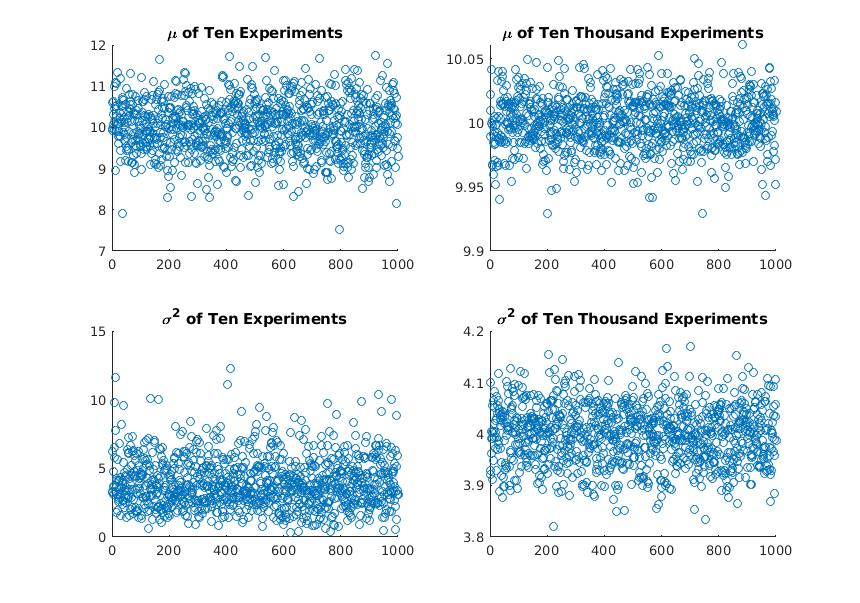
\includegraphics[width=\textwidth]{scatterPlots.jpg}
                \caption{Scatter plot of means and variances of all realisations}
                \label{fig:scatters}
            \end{figure}

            \begin{figure}[!ht]
                \centering
                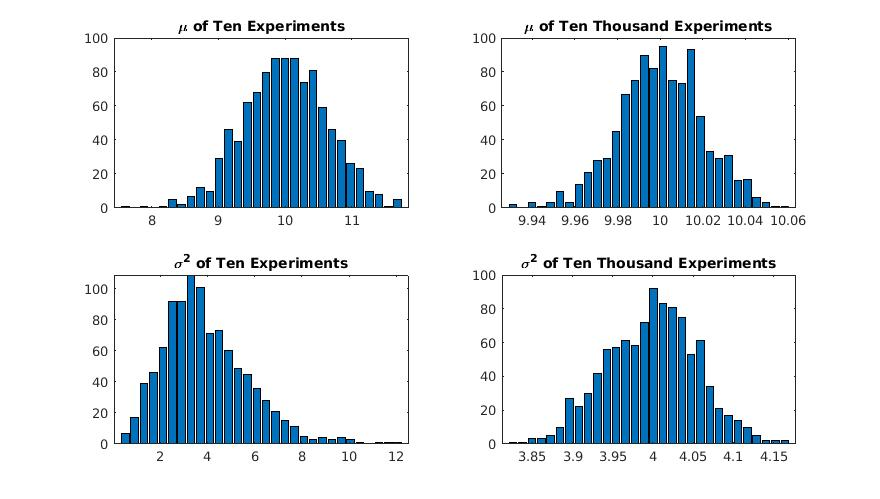
\includegraphics[width=\textwidth]{pdfOfMeansAndStdDev.jpg}
                \caption{Distributions of means and variances of all realisations}
                \label{fig:dists}
            \end{figure}

            From the plots in \cref{fig:dists,fig:scatters} it can be seen that the realisations of 10 samples has a wider distribution spanning whole integers, and the realisations of 10000 samples, which spans a range 100 times smaller. All of these, aside from the distribution of the variance for 10 samples appear to have a normal distribution. The outlier has a right skew to the distribtion, which is visible in the scatter plot as there is a dense cluster and a thinner set of points above it, opposed to the other plots which have a dense cluster in the middle and thin tails either side. This indicates that the increase in samples per random variable makes the variance more normally distributed.
            \par
            One of the differences between the two sets of realisations is the range that they are over. The set with 10 samples is over whole integers and the set with 10000 is over a range 100 times smaller. We know this to be true as the increase in samples reduces the standard deviation by a factor of $\sqrt{N}$ which can be seen in he 10000 set is $\sqrt{10000} = 100$, this also has an effect on the variance. According to \cite{sampling_dists_2020}, the sampled variance of a normally distributed random variable is $\chi^2$ distributed with $N-1$ degrees of freedom. Which can be seen from the fact that we know that the lower the degrees of freedom the more right skew the distribution has, and at 9999 degrees of freedom the $\chi^2$ becomes more centered, like that of the variances distribution for 10000 samples (\cref{app:chiDists}). This can also be explained by the central limit theorem, by summing the $\chi^2$ distributions together, it results in a normal distribution that approximates it.


        \subsection{Speech}

            \begin{figure}[!ht]
                \centering
                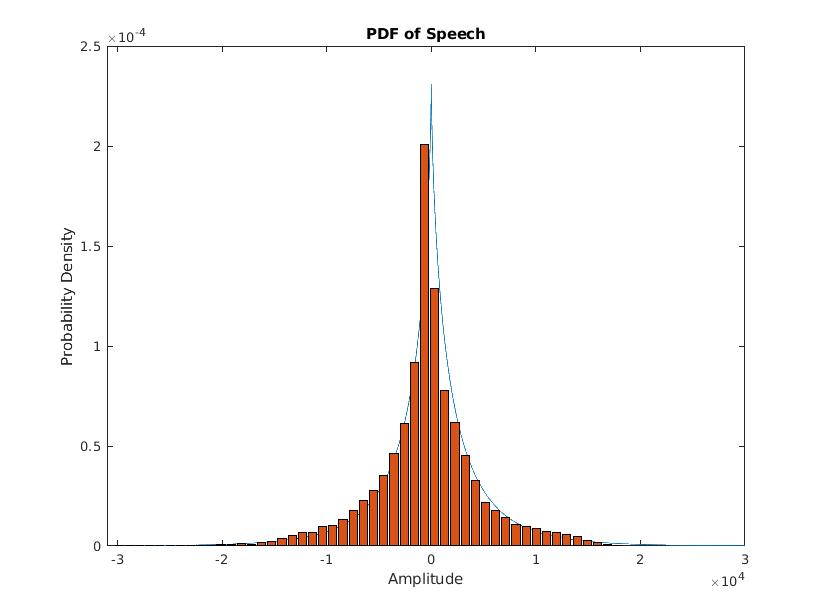
\includegraphics[width=\textwidth]{PDF_of_speech.jpg}
                \caption{Distribution of the speech signal}
                \label{fig:speech}
            \end{figure}

            With the initial approximation that $\alpha = \sqrt{2\sigma^2} = 6978.9$, we can find the value that maximises $\beta$ by comparing the outputs of various $\beta$ values, resulting in a first $\beta = 1.62$. Using this value of $\beta$, we can then find a value of $\alpha$ that maximises the new function, doing this results in $\alpha = 5868.6$. Continuing with this maximisations for each value one at a time, until it converges results in a final parameter pair $\theta = [\alpha = 1727.1, \beta = 0.707]$.
            \par
            The PDF for the converged values of $\alpha$ and $\beta$ is the blue line plotted in \cref{fig:speech}. Alongside this is the PMF of speech signal is plotted in orange. We can see that these two line up pretty well, indicating that the distribution from the found values is close to or exactly the distribution of this speech signal. This distribution is in the Laplace family of distributions.
            

    \section{Conclusion}
        From esimating statistics for a series of gaussian random variables, we can see that as we increase the number of samples in a realisation the more accurate our estimate of the mean and variance are. It is also seen that the distribution becomes more normally distributed with more samples.
        \par
        Additionally, we have seen an outline for a method of approximating the distribution of a speech signal. We do this by computing the maximum likelihood estimation by maximising both $\alpha$ and $\beta$ one after the other until they both converge. From here we can see that the distribution estimated is a laplacian distribution that comes very close to the distribution of the signal and is a good model for this signal.     


    % \Urlmuskip=0mu plus 1mu\relax
    \bibliography{bibliography}
    \bibliographystyle{IEEEtran}

    \begin{appendices}
        \section{$\chi^2$ Distributions}
        \label{app:chiDists}
            \begin{figure}[!ht]
                \centering
                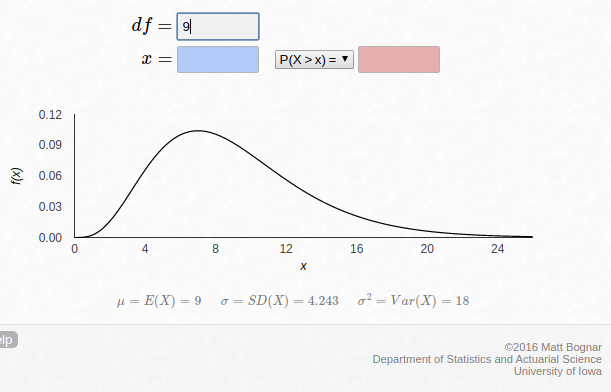
\includegraphics[width=\textwidth]{nu9.png}
                \caption{$\chi^2$ distribution with $\nu=9$}
            \end{figure}
            \begin{figure}[!ht]
                \centering
                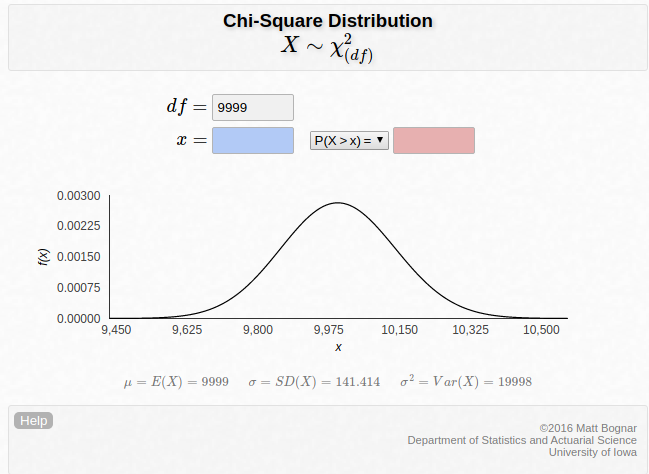
\includegraphics[width=\textwidth]{nu9999.png}
                \caption{$\chi^2$ distribution with $\nu=9999$}
            \end{figure}
        \section{MATLAB code for Gaussian Random Variables}
            \lstinputlisting{../q1.m}
        \section{MATLAB code for Speech Estimation}
            \lstinputlisting{../q2.m}
    \end{appendices}
\end{document}